\documentclass[mathserif]{beamer}

\usepackage{subg}

%-----------------------------------------------------------------------
\usepackage{pdfpages}
\usepackage{array}
\usepackage{booktabs}
\usepackage[skins,breakable]{tcolorbox}
\usepackage{minibox}
\usepackage{mathtools}
\usepackage{amsmath}

% Avoid random transparencies in Adobe Acrobat
\usepackage{everypage}
\AddEverypageHook{%
  \makeatletter%
  \special{pdf: put @thispage <</Group << /S /Transparency /I true /CS /DeviceRGB>> >>}%
  \makeatother%
}%

\DeclareMathOperator*{\argmax}{arg\,max}

\newcommand{\todo}[1]{{\scriptsize\color{yellow}\textsc{[Todo]}}}

\newcommand{\qcite}[1]{{\scriptsize\color{col1}[#1]}}

\newcommand{\qbox}[1]{%
\begin{tcolorbox}[enhanced jigsaw,size=tight,hbox,boxsep=4pt,boxrule=1pt,coltext=black,colframe=col1light,colback=col1,opacityback=0.7,opacityframe=1]
\strut #1
\end{tcolorbox}%
}

\newcommand{\qboxa}[1]{%
\begin{tcolorbox}[enhanced jigsaw,size=tight,hbox,boxsep=4pt,boxrule=1pt,coltext=textcolor,colframe=col1,opacityback=0,opacityframe=1]
\strut #1
\end{tcolorbox}%
}

\newcommand{\qboxatight}[1]{%
\begin{tcolorbox}[enhanced jigsaw,size=fbox,hbox,boxsep=4pt,boxrule=1pt,coltext=textcolor,colframe=col1,opacityback=0,opacityframe=1,halign=center,valign=center,square,circular arc]
#1
\end{tcolorbox}%
}

\newcommand{\qboxb}[1]{%
\begin{tcolorbox}[enhanced jigsaw,size=tight,hbox,boxsep=4pt,boxrule=1pt,coltext=textcolor,colframe=col2,opacityback=0,opacityframe=1]
\strut #1
\end{tcolorbox}%
}

\newcommand{\qtheorem}[2]{%
\begin{tcolorbox}[enhanced jigsaw,size=tight,boxsep=7pt,boxrule=0.7pt,coltext=textcolor,colframe=col1,colback=col1,opacityback=0,opacityframe=1]
\begin{minipage}{\textwidth}
{\color{col1}\strut Theorem #1}\\[0.7em]
#2
\end{minipage}
\end{tcolorbox}%
}

\newcommand{\qlemma}[1]{%
\begin{tcolorbox}[enhanced jigsaw,size=tight,boxsep=7pt,boxrule=0.7pt,coltext=textcolor,colframe=col2,colback=col1,opacityback=0,opacityframe=1]
\begin{minipage}{\textwidth}
{\color{col2}\strut Lemma}\\[0.7em]
#1
\end{minipage}
\end{tcolorbox}%
}

\newcommand{\qsubtitle}[1]{%
{\color{col2}\textsc{#1}}
}
%-----------------------------------------------------------------------

\title[Discrete Sampling using Semigradient-based Product Mixtures]
{Discrete Sampling using Semigradient-based Product Mixtures}

\author[Alkis Gotovos]{}

\begin{document}

\setbeamertemplate{background canvas}{}
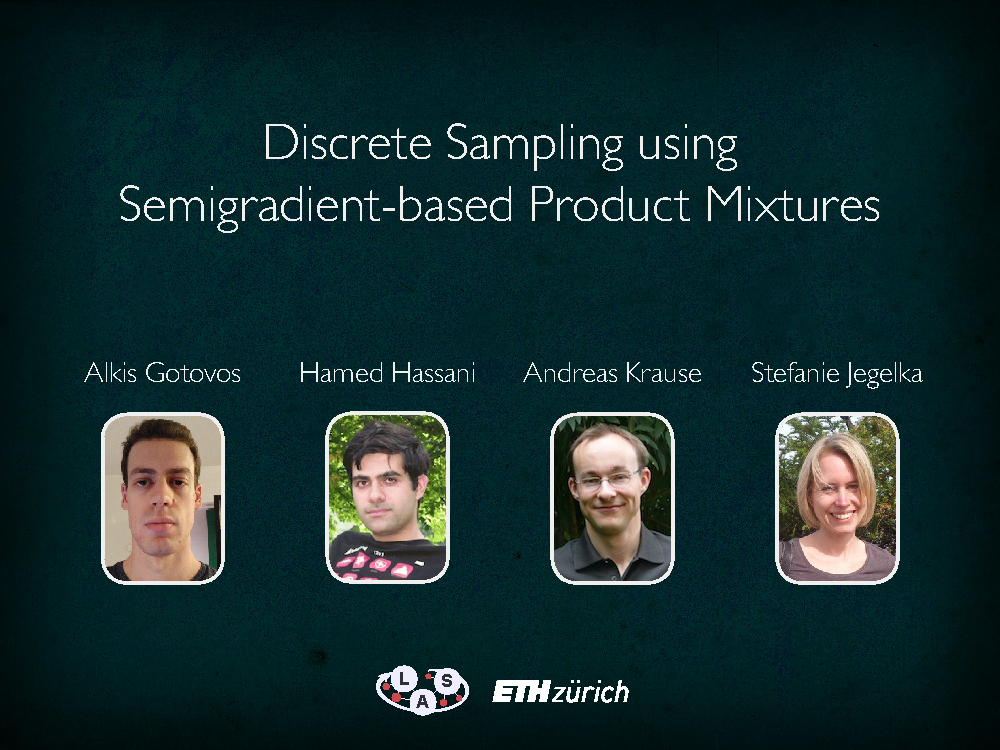
\includepdf[pages={1}]{title/title.pdf}
\setbeamertemplate{background canvas}{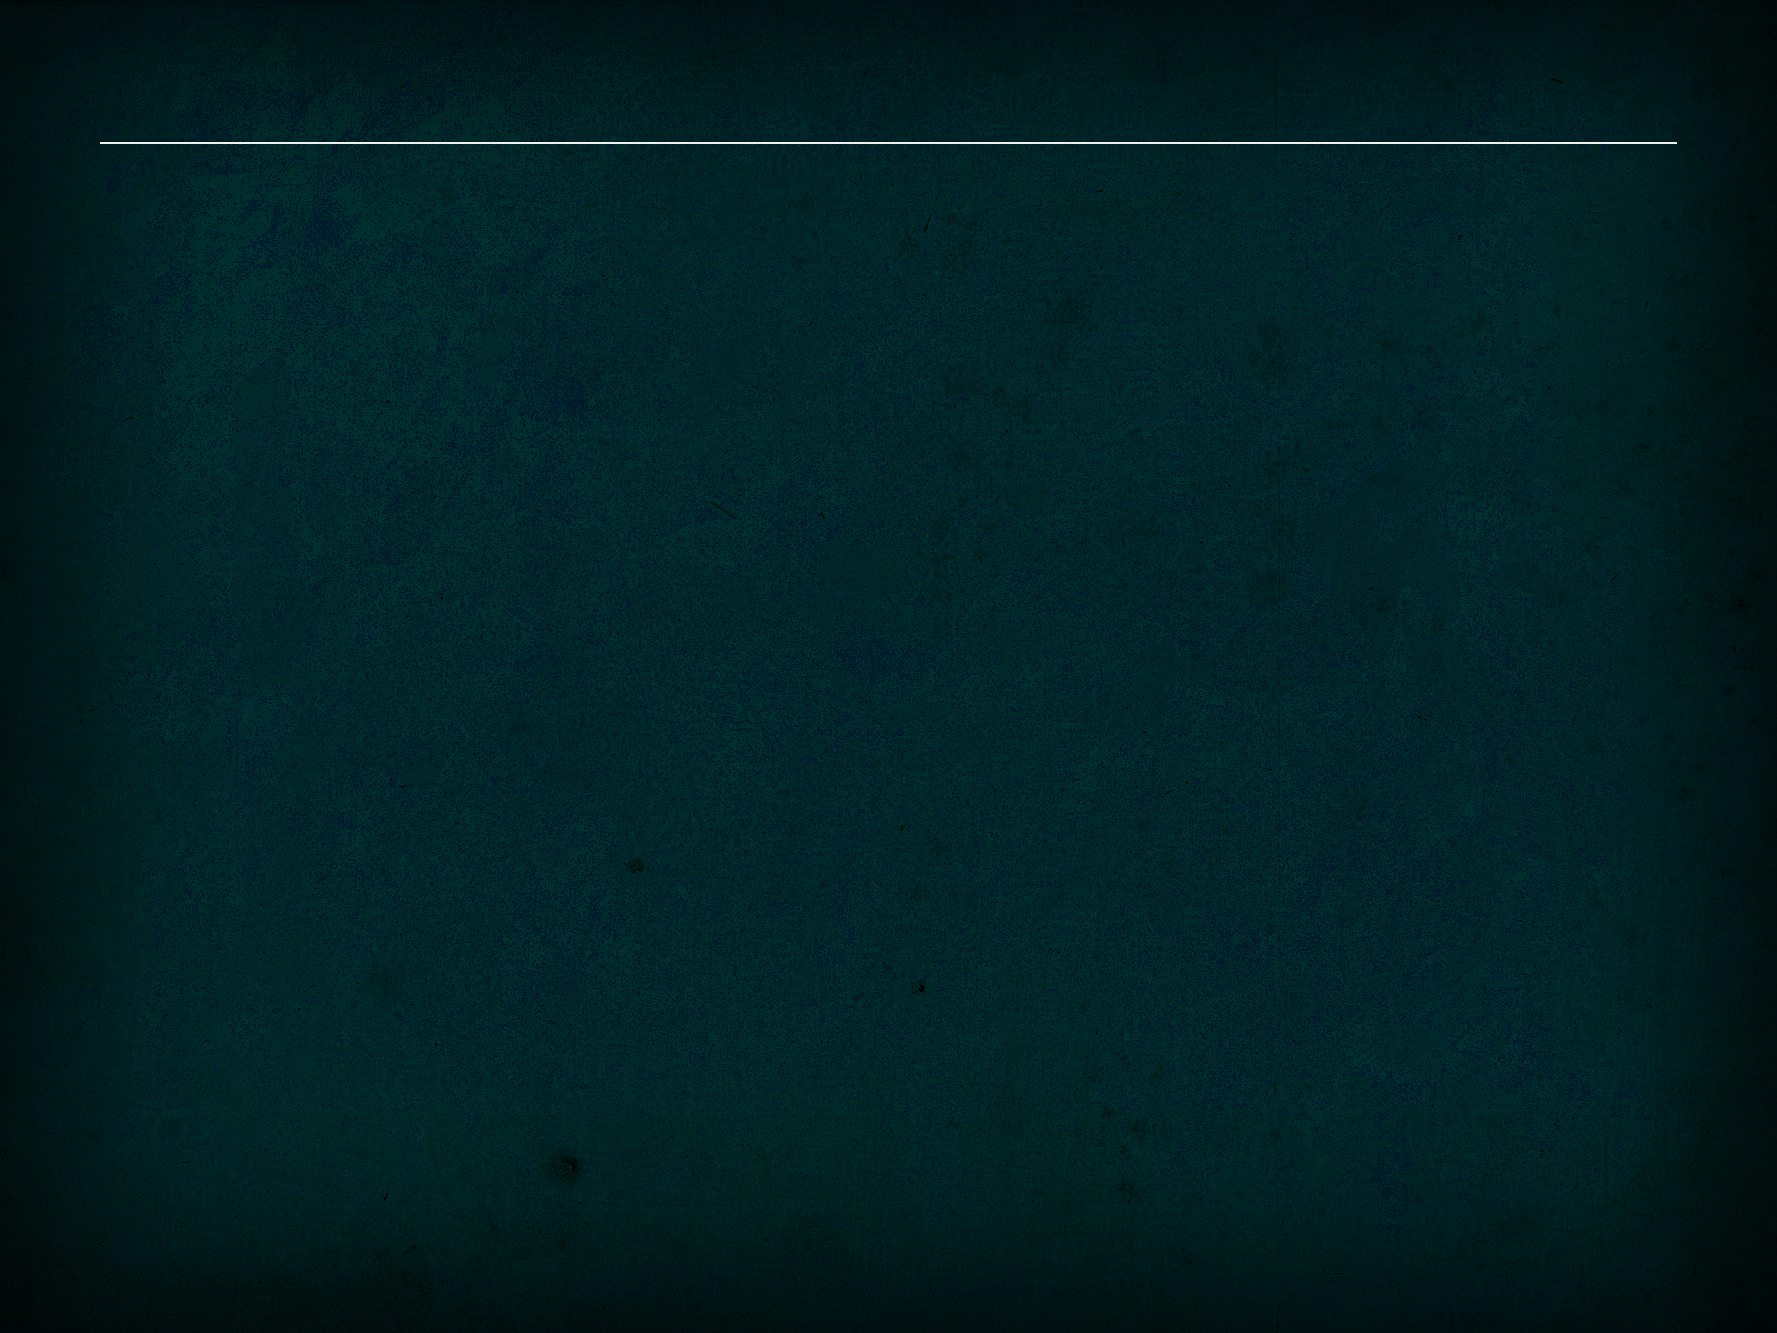
\includegraphics[width=\paperwidth]{figures/bg.png}}

\begin{frame}{Introduction}
\vspace{0.2in}
\centering

\includegraphics[width=\textwidth]{figures/champions_transparent.png}
\end{frame}

\begin{frame}{Introduction}
\vspace{0.2in}
\centering
\begin{columns}
\begin{column}{0.3\textwidth}
\hfill
\includegraphics[width=1.2in]{figures/ssg_new.png}
\end{column}
\begin{column}{0.1\textwidth}
\centering
{\Large vs.}
\end{column}
\begin{column}{0.3\textwidth}
\includegraphics[width=1.2in]{figures/skt_new.png}
\hfill
\end{column}
\end{columns}
\end{frame}

\begin{frame}{Introduction}
\vspace{0.2in}
\centering
\begin{columns}
\column{0.3\textwidth}
\only<1>{\includegraphics[width=1.2in]{figures/ssg_partial1.png}}%
\only<2-4>{\includegraphics[width=1.2in]{figures/ssg_partial2.png}}%
\only<5->{\includegraphics[width=1.2in]{figures/ssg_partial3.png}}
\column{0.6\textwidth}
\begin{itemize}
\item<3-> Ground set $V$\\[0.5em]

\includegraphics[width=2in]{figures/champions_transparent.png}
\vspace{2em}
\item<4-> Score function $F : 2^V \to \mathbb{R}$
\vspace{2em}
\item<6-> $(d, e) = \displaystyle\argmax_{({\color{col1}x}, {\color{col1}y}) \in V \times V} F(\{a, b, c, {\color{col1}x}, {\color{col1}y}\})$
\end{itemize}
\end{columns}
\end{frame}

\begin{frame}{Discrete probabilistic models}
\begin{itemize}
\item Multiple suggestions \uncover<4->{$\ \ \longrightarrow\ \ $ sample from $p\left(S \mid S \supseteq \{a, b, c\}\right)$}
\vspace{1.5em}
\item<2-> Learn $F$ from data \uncover<5->{$\ \ \ \,\longrightarrow\ \ $ max. likelihood}
\end{itemize}
\vspace{3em}
\centering
\uncover<3->{\qboxa{
$p(S) = \displaystyle\frac{1}{Z} \exp(F(S))$
}
}
\end{frame}

\begin{frame}{Ising model}
\vspace{0.2in}
\centering
\only<1>{\includegraphics[width=3in]{figures/ising.png}}%
\only<2>{\includegraphics[width=3in]{figures/ising5.png}}%
\only<3>{\includegraphics[width=3in]{figures/ising5_cut.png}}%
\only<4->{\includegraphics[width=3in]{figures/ising5_cut_fij.png}}

\vspace{1em}
\uncover<5>{
$F(S) = \displaystyle\sum_{i \sim j} F_{ij}(S)$
}
\end{frame}

\begin{frame}{Higher-order interactions}
\vspace{0.2in}
\centering
\only<1>{\includegraphics[width=3in]{figures/ising_higher.png}}%
\only<2->{%
\begin{columns}
\column{0.3\textwidth}
\centering
\includegraphics[width=1.7in]{figures/ising_higher.png}
\column{0.69\textwidth}
\centering
\includegraphics[width=2.3in]{figures/concave_over_modular.pdf}
\end{columns}
}
\vspace{3em}
\uncover<3>{%
$F(S) = \phi(|S \cap V_i|) + \ldots$
}
\end{frame}

\begin{frame}{Probabilistic submodular models}
\centering
\qboxa{
$p(S) = \displaystyle\frac{1}{Z} \exp(F(S))$
}
\vspace{2em}
$F : 2^V \to \mathbb{R}$ is a submodular or supermodular function
\end{frame}

\begin{frame}{Landscape of models}
\vspace{0.1in}
\centering
\only<1>{\includegraphics[width=4.3in]{figures/venn01.pdf}}%
\only<2>{\includegraphics[width=4.3in]{figures/venn02.pdf}}%
\only<3>{\includegraphics[width=4.3in]{figures/venn03.pdf}}%
\only<4>{\includegraphics[width=4.3in]{figures/venn04.pdf}}%
\only<5>{\includegraphics[width=4.3in]{figures/venn06.pdf}}%
\only<6>{\includegraphics[width=4.3in]{figures/venn07.pdf}}%
\only<7>{\includegraphics[width=4.3in]{figures/venn08.pdf}}
\end{frame}

\begin{frame}{Inference}
\vspace{1em}

\begin{minipage}{\textwidth}
\begin{columns}[c]
\column{0.43\textwidth}
\includegraphics[width=1.85in]{figures/inf01_exact_horz.pdf}
\column{0.57\textwidth}
\begin{itemize}
\item \small{Tractable only for limited subclasses}
\vspace{1em}
\item \small{\#P-hard even for Ising models}
\end{itemize}
\end{columns}
\end{minipage}

\uncover<2->{
\vspace{2em}
\begin{minipage}{\textwidth}
\begin{columns}[c]
\column{0.43\textwidth}
\includegraphics[width=1.85in]{figures/inf02_loworder_horz.pdf}
\column{0.57\textwidth}
\begin{itemize}
\item \small{Extensively studied model class}
\vspace{1em}
\item \small{Complexity exponential in model order}
\end{itemize}
\end{columns}
\end{minipage}
}

\uncover<3->{
\vspace{2em}
\begin{minipage}{\textwidth}
\begin{columns}[c]
\column{0.43\textwidth}
\includegraphics[width=1.85in]{figures/inf03_psm_horz.pdf}
\column{0.57\textwidth}
\begin{itemize}
\item \small{Variational approach for general PSMs}\\\qcite{Djolonga and Krause, '14}\\\qcite{Djolonga et al., '16}
\end{itemize}
\end{columns}
\end{minipage}
}
\end{frame}

\begin{frame}{Inference}
\centering
\includegraphics[width=2in]{figures/venn08.pdf}
\vspace{0.5em}
\centering
\qboxa{\large \strut What about sampling?}
\vspace{1em}
\begin{itemize}
\item<2-> Under what conditions is the Gibbs sampler efficient?\\
          \qcite{G., Hassani and Krause, '15}
\vspace{1em}
\item<3-> Can we come up with improved sampling schemes?\\
          \qcite{G., Jegelka, Hassani and Krause, '17}
\end{itemize}
\end{frame}

\begin{frame}{Markov chain Monte Carlo}
\begin{tabular}{*{2}{@{}l}}
\begin{minipage}{0.45\textwidth}
\begin{itemize}
\item<1-> State space $\Omega$
\end{itemize}
\end{minipage} & \uncover<3->{\color{col1}powerset of $V$}\\[1.5em]
\begin{minipage}{0.45\textwidth}
\begin{itemize}
\item Transition matrix $P$
\end{itemize}
\end{minipage} & \uncover<4->{\color{col1}Gibbs sampler}\\[1.5em]
\begin{minipage}{0.45\textwidth}
\begin{itemize}
\item Stationary distribution $\pi$
\end{itemize}
\end{minipage} & \uncover<5->{\color{col1}$\pi(S) \propto \exp(F(S))$}
\end{tabular}

\uncover<2->{
\vspace{3em}
Markov chain $\left(S_t\right)_{t \geq 0}$ that moves according to $P$
}
\end{frame}

\begin{frame}{Gibbs sampler}
\vspace{1em}
\centering
\includegraphics[height=2.7in]{figures/lattice_nodes_only.pdf}
\end{frame}

\begin{frame}{Gibbs sampler}
\vspace{1em}
\begin{columns}[c]
\column{0.5\textwidth}
\uncover<2->{Start at $S_0$

\vspace{1.1em}
For $t = 1, 2, \ldots$}
\vspace{1.1em}
\begin{itemize}
\item<4-> Select random $v \in V$
\vspace{1.1em}
\item<7-> Compute conditional $p_{\textrm{add}}$
\vspace{1.1em}
\item<8-> Flip biased coin

\vspace{-1em}
\begin{minipage}{0.5\textwidth}\vspace{2em}\includegraphics[width=2.5in]{figures/gibbs.pdf}\end{minipage}
\end{itemize}
\column{0.5\textwidth}
\only<1-2>{\includegraphics[height=2.5in]{figures/lattice_nodes_only_large.pdf}}%
\only<3-4>{\includegraphics[height=2.5in]{figures/lattice_example_node.pdf}}%
\only<5>{\includegraphics[height=2.5in]{figures/lattice_example_edges.pdf}}%
\only<6-7>{\includegraphics[height=2.5in]{figures/lattice_example_edges_one.pdf}}%
\only<8>{\includegraphics[height=2.5in]{figures/lattice_example_edges_one_trans.pdf}}
\vspace{2em}
\end{columns}
\end{frame}

\begin{frame}{Mixing time}
\vspace{0.5em}
\qboxa{Does the Markov chain converge?}

\vspace{0.5em}
\only<2->{Total variation distance}
\only<2>{
\begin{align*}
d(t) = d_{\mathrm{tv}}\left(\mathbb{P}_{S_t}, \pi\right)
\end{align*}}
\only<3>{
\begin{align*}
d(t) = {\color{col1}\max \{}d_{\mathrm{tv}}\left(\mathbb{P}_{S_t}, \pi\right) {\color{col1}\mid S_0 \in \Omega\}}
\end{align*}
}
\alt<1,4->{\uncover<4->{
\begin{align*}
d(t) = \max \{d_{\mathrm{tv}}\left(\mathbb{P}_{S_t}, \pi\right) \mid S_0 \in \Omega\}
\end{align*}
}}{}

\uncover<4->{
\vspace{-1em}
Under mild assumptions (ergodicity), $\ \ d(t) \xrightarrow{\ t\,\rightarrow\,\infty\ } 0$
}

\uncover<5->{
\vspace{2.5em}
\qboxa{How long does it take to get ``close enough" to $\pi$?}
}

\uncover<6->{
\vspace{1em}
Mixing time $\ \ \ t_{\textrm{mix}}(\epsilon) = \min \left\{t \mid d(t) \leq \epsilon \right\}$
}
\end{frame}

\begin{frame}{Mixing time}
\begin{itemize}
\item<1-> Mixing times for general PSMs are exponential in $|V| = n$
\vspace{1em}
\item<2-> Exponential even for pairwise models \qcite{Jerrum and Sinclair, '93}
\end{itemize}

\uncover<3->{
\vspace{3em}
\centering
\qboxa{\minibox{We establish sufficient conditions for sub-exponential mixing\\of the Gibbs sampler on PSMs.}}
}
\end{frame}

\begin{frame}{Polynomial-time mixing}
\vspace{0.5em}
\only<1>{\includegraphics[width=3.9in,trim=5 0 0 0,clip]{figures/ineq_mod_0.pdf}}%
\only<2>{\includegraphics[width=3.9in,trim=5 0 0 0,clip]{figures/ineq_mod_1.pdf}}%
\only<3->{\includegraphics[width=3.9in,trim=5 0 0 0,clip]{figures/ineq_mod_2.pdf}}

\uncover<4->{
\vspace{4em}
``Distance" from modularity
\begin{align*}
\uncover<5->{\zeta_F \coloneqq \max_{A, B \subseteq V}} \uncover<4->{\big|F(A) + F(B) - F(A \cup B) - F(A \cap B)\big|}
\end{align*}
}
\end{frame}

\begin{frame}{Polynomial-time mixing}
\qtheorem{1}{
For any submodular or supermodular set function $F$, the mixing time of the Gibbs sampler is bounded by
\begin{align*}
t_{\textrm{mix}}(\epsilon) = \mathcal{O}\left(n^2 \exp(\zeta_F)\log\epsilon^{-1}\right).
\end{align*}
}
\end{frame}

\begin{frame}{When Gibbs fails}
\centering
\only<1>{\includegraphics[width=4in]{figures/ising_hard0.pdf}}%
\only<2>{\includegraphics[width=4in]{figures/ising_hard1.pdf}}%
\only<3>{\includegraphics[width=4in]{figures/ising_hard2.pdf}}
\end{frame}

\begin{frame}{When Gibbs fails}
\centering
\only<1>{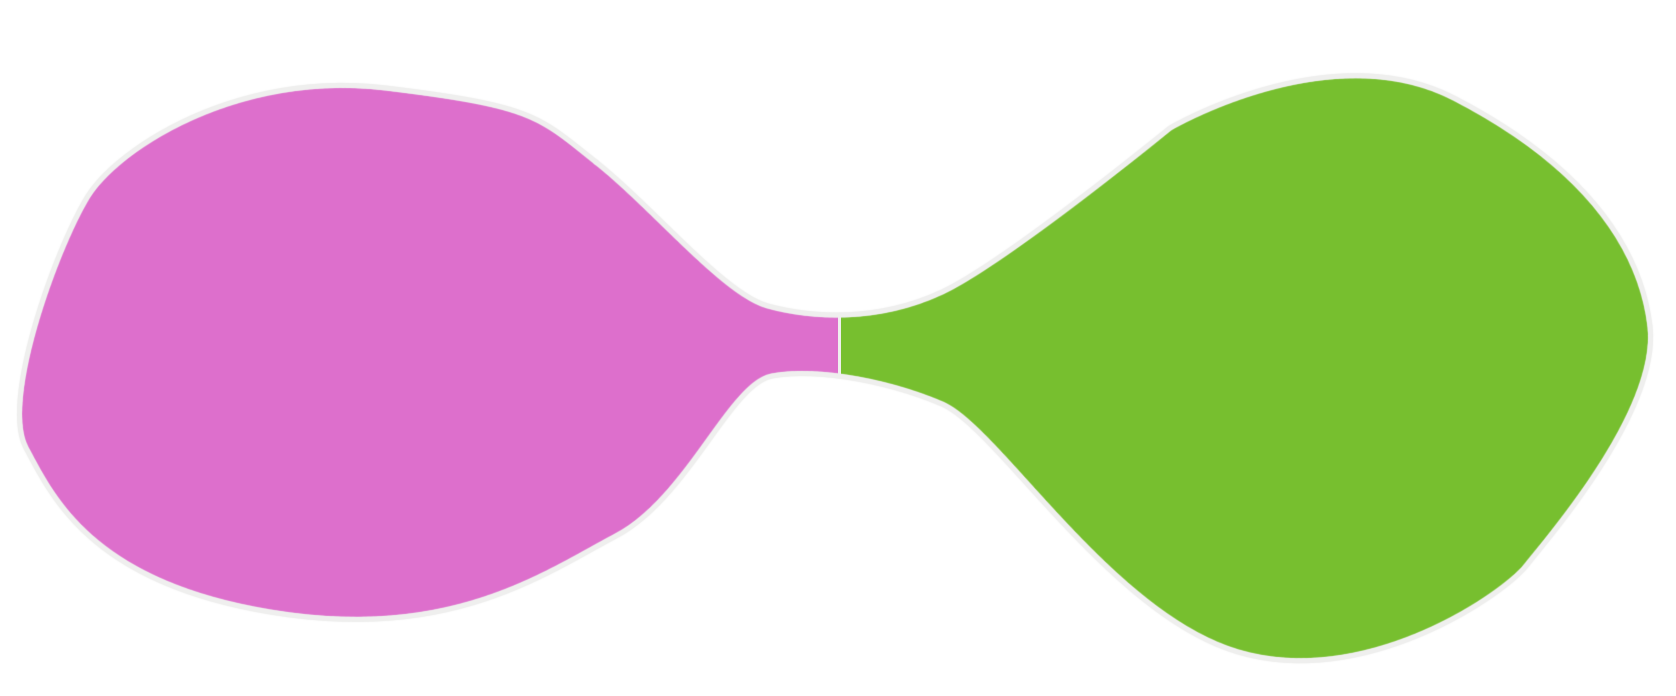
\includegraphics[width=4in]{figures/bottleneck1.png}}%
\only<2>{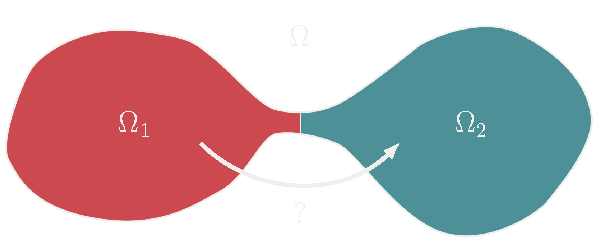
\includegraphics[width=4in]{figures/bottleneck2.png}}%
\only<3>{\includegraphics[width=4in]{figures/bottleneck3.pdf}}
\end{frame}

\begin{frame}{The $\mathrm{M}^3$ chain}
\vspace{0.2in}
Start at $S_0$

\vspace{1.1em}
For $t = 1, 2, \ldots$
\vspace{1.1em}
\begin{itemize}
\item<2-> Sample $R \sim q(S_t, R)$
\vspace{1.1em}
\item<3-> Compute $p_{\mathrm{accept}} = \min \left\{1, \frac{\pi(R)q(S_t, R)}{\pi(S)q(R, S_t)}\right\}$
\vspace{1.1em}
\item<4-> Flip biased coin

\vspace{-1em}
\begin{minipage}{0.5\textwidth}\vspace{2em}\includegraphics[width=2.5in]{figures/metropolis.pdf}\end{minipage}
\end{itemize}
\end{frame}

\begin{frame}{The $\mathrm{M}^3$ chain}
\begin{columns}
\column{0.55\textwidth}
\begin{itemize}
\item Proposal distribution\\[0.5em]
\only<1>{$q(S, R) = \displaystyle\frac{1}{Z_q} \sum_{i = 1}^r w_i \exp\left(m_i(R)\right)$}%
\only<2>{$q({\color{col1}R}) = \displaystyle\frac{1}{Z_q} \sum_{i = 1}^r \exp\left(m_i(R)\right)$}%
\only<3->{$q(R) = \displaystyle\frac{1}{Z_q} \sum_{i = 1}^r \exp\left(m_i(R)\right)$}\\[2.5em]
\item<4-> \only<4>{Each $m_i$ is a modular function\\[0.5em]
$m_i(R) = \sum_{v \in R} m_{iv}$\\[2.5em]}%
\only<5-6>{Each $m_i$ is a {\color{col1}sub-/supergradient of $F$}\\[0.5em]
$m_i(R) = \sum_{v \in R} m_{iv}$\\[2.5em]}%
\only<7->{Each $m_i$ is a sub-/supergradient of $F$\\[0.5em]
$m_i(R) = \sum_{v \in R} m_{iv}$\\[2.5em]}
\item<7-> Combine Gibbs and $\mathrm{M}^3$\\[0.5em]
$P^{\mathrm{combo}} = \alpha P^{\mathrm{Gibbs}} + (1-\alpha) P^{\mathrm{M^3}}$
\end{itemize}
\column{0.44\textwidth}
\uncover<6->{\includegraphics[width=1.65in]{figures/subgradient.pdf}}
\end{columns}
\end{frame}

\begin{frame}{Decomposition theorem \qcite{Jerrum et al., '04}}
\vspace{1em}
\centering
\only<1>{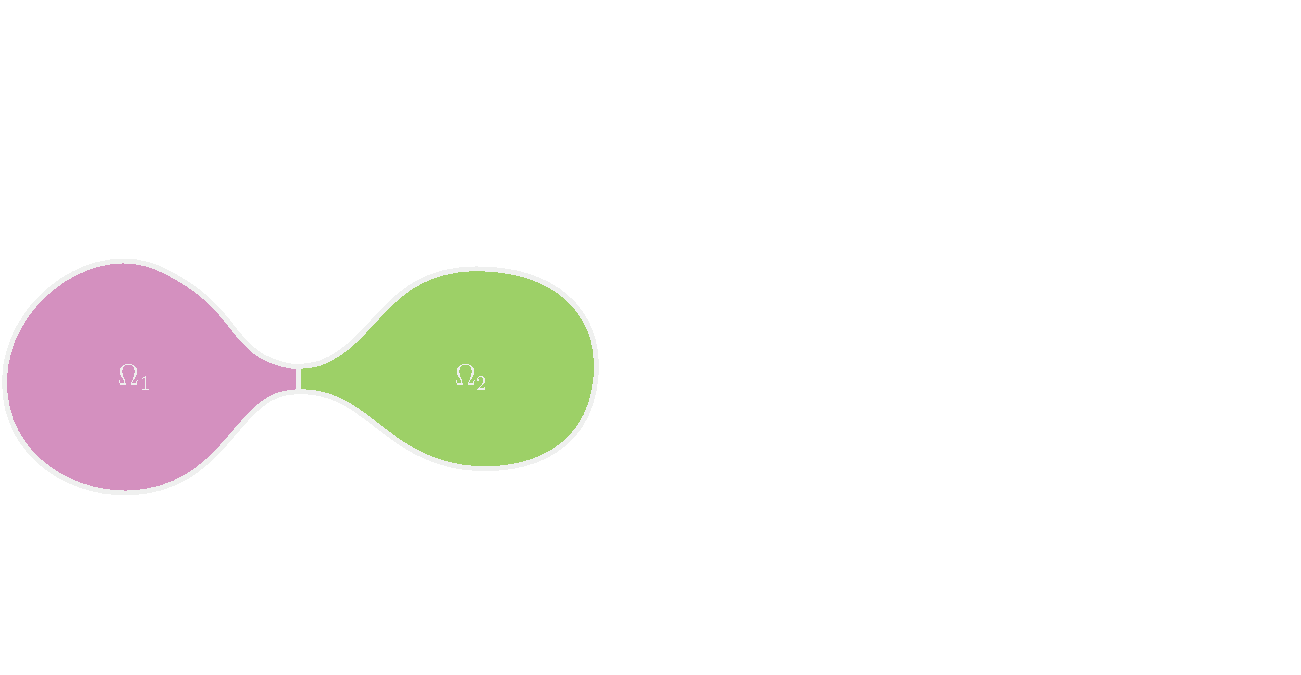
\includegraphics[width=4.2in]{figures/decomposition1.pdf}}%
\only<2>{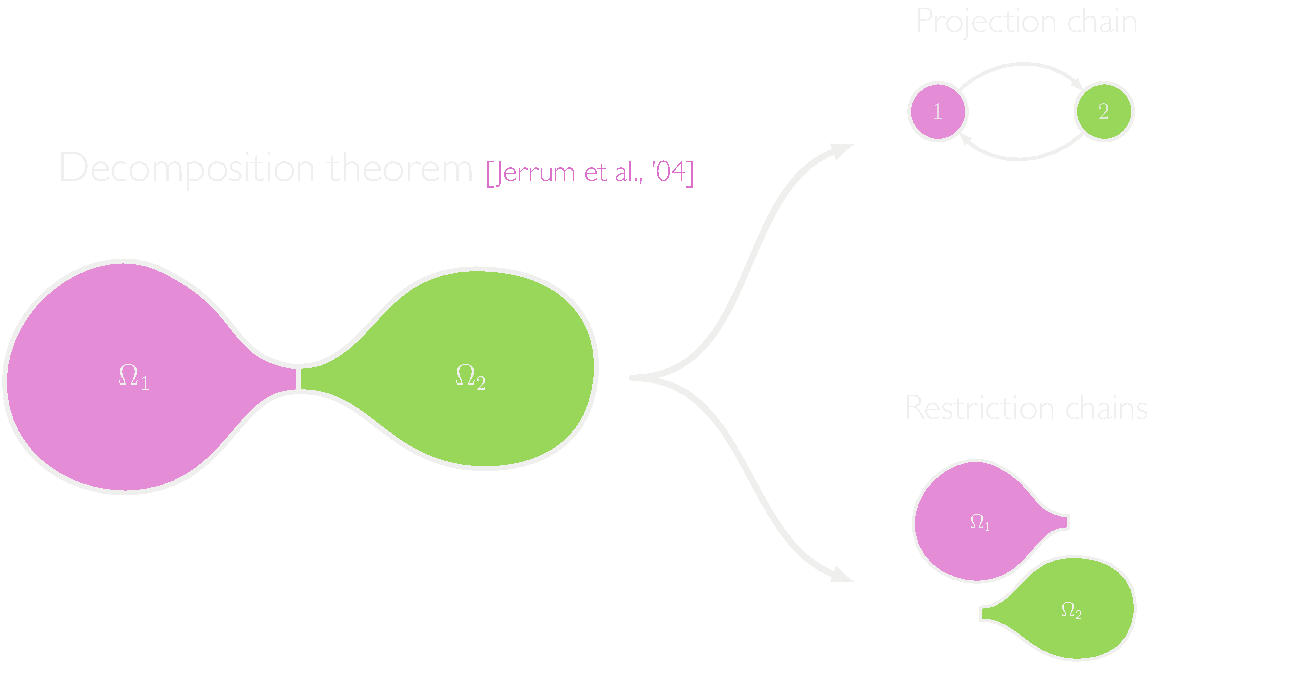
\includegraphics[width=4.2in]{figures/decomposition2.pdf}}%
\only<3>{\includegraphics[width=4.2in]{figures/decomposition3.pdf}}%
\only<4>{\includegraphics[width=4.2in]{figures/decomposition4.pdf}}%
\only<5->{\includegraphics[width=4.2in]{figures/decomposition5.pdf}}\\[0.1em]
\end{frame}

\begin{frame}{Decomposition theorem \qcite{Jerrum et al., '04}}
\begin{center}
\includegraphics[width=2.5in]{figures/decomposition5.pdf}
\end{center}

For a specific class of Ising models, we show:\\[1em]
\begin{itemize}
\item Gibbs $\ \ \ \ \ \ t_{\textrm{mix}}(\epsilon) = \Omega\left( e^{cn}\log(\epsilon^{-1}) \right)$\\[1em]
\item Combo $\ \ \ t_{\textrm{mix}}(\epsilon) = \mathcal{O}\left( n^2 \log(\epsilon^{-1}) \right)$
\end{itemize}
\end{frame}

\begin{frame}{Evaluation}
\centering
\includegraphics[width=2in]{figures/hots_logo.png}\\[1em]

\begin{itemize}
\item Data set: $8.5$k teams of $5$ characters\\[1em]
\item<2-> $|V| = 48$\\[1em]
\item<3-> $F$ is a log-submodular facility location (FLID) model \qcite{Tschiatschek et al., '16}\\[1em]
\item<4-> Subgradients drawn either randomly or incrementally
\end{itemize}
\end{frame}

\begin{frame}{Evaluation}
\vspace{0.25in}
\centering
\only<1>{\includegraphics[width=4.1in,trim=0 0 0 0,clip]{figures/hots1.pdf}}%
\only<2>{\includegraphics[width=4.1in,trim=0 0 0 0,clip]{figures/hots1_line.pdf}}%
\only<3>{\includegraphics[width=4.1in,trim=0 0 0 0,clip]{figures/water2.pdf}}%
\only<4>{\includegraphics[width=4.1in,trim=0 0 0 0,clip]{figures/water3.pdf}}%
\end{frame}

\begin{frame}{Evaluation}
\vspace{0.05in}
\centering
\includegraphics[width=3.2in]{figures/hots.pdf}
\end{frame}

\begin{frame}{Conclusion}
\vspace{0.2in}
\begin{columns}[c]
\column{0.45\textwidth}
\centering
\includegraphics[height=2.6in]{figures/bee_marginals.png}\\[0.3em]
\qcite{Djolonga and Krause, '15}
\column{0.55\textwidth}
\centering
\uncover<2->{\includegraphics[height=2.6in]{figures/flickr_inference.pdf}\\[0.3em]
\qcite{Tschiatschek et al., '16}}
\end{columns}
\end{frame}

\begin{frame}{Conclusion}
\vspace{0.1in}
\only<1>{\includegraphics[width=4.3in]{figures/venn07_1.pdf}}%
\only<2>{\includegraphics[width=4.3in]{figures/venn_rayleigh.pdf}}
\end{frame}
\end{document}
